\begin{figure}[h]
  \centering
  {\fbox{
      $\begin{array}{c}

         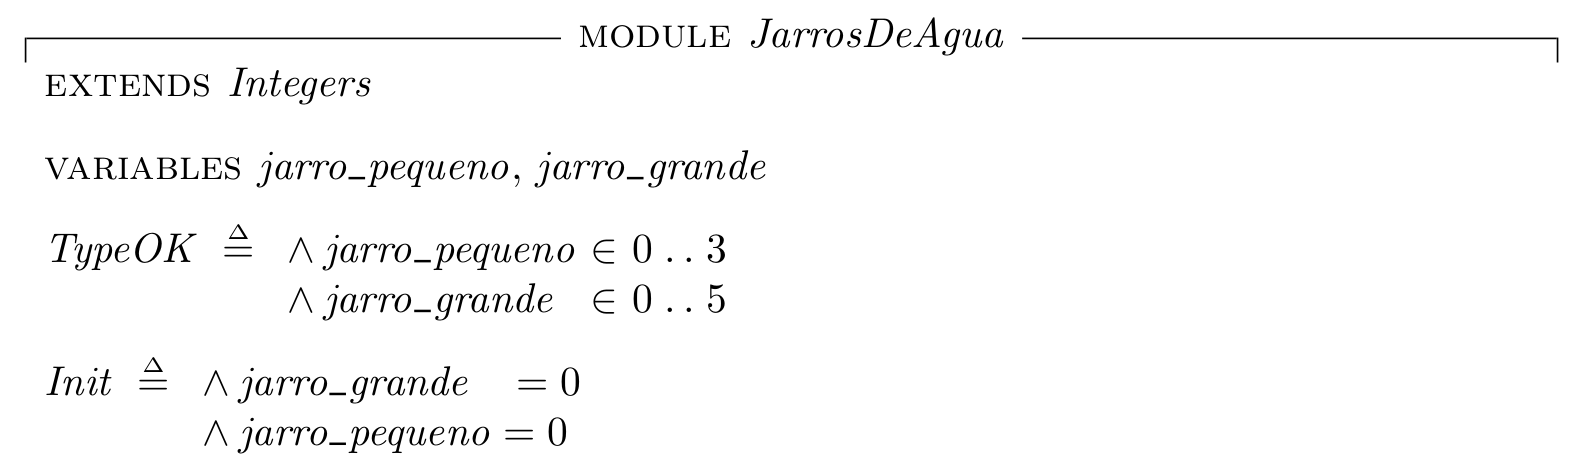
\includegraphics[width=0.9\textwidth]{JarrosP1.png}\\

         \TEqD\ (\texttt{MOD})\\

         \progfigmed{
         defmodule JarrosDeAgua do\\
         ~~require Oracle\\
         ~~@oracle spawn(Oracle, :listen, [])\\
         ~~ ...\\
         end\\
         \\
         JarrosDeAgua.main(\\
         ~~\%\{\\
         ~~~~jarro\_grande: 0,\\
         ~~~~jarro\_pequeno: 0\\
         ~~\}\\
         )
         }
        
       \end{array}$
     }}
   \caption{Tradução do módulo Jarros de Água}
   \label{fig:jarros-ex-mod}
 \end{figure}

 \begin{figure}[h]
  \centering
  {\fbox{
      $\begin{array}{c}

         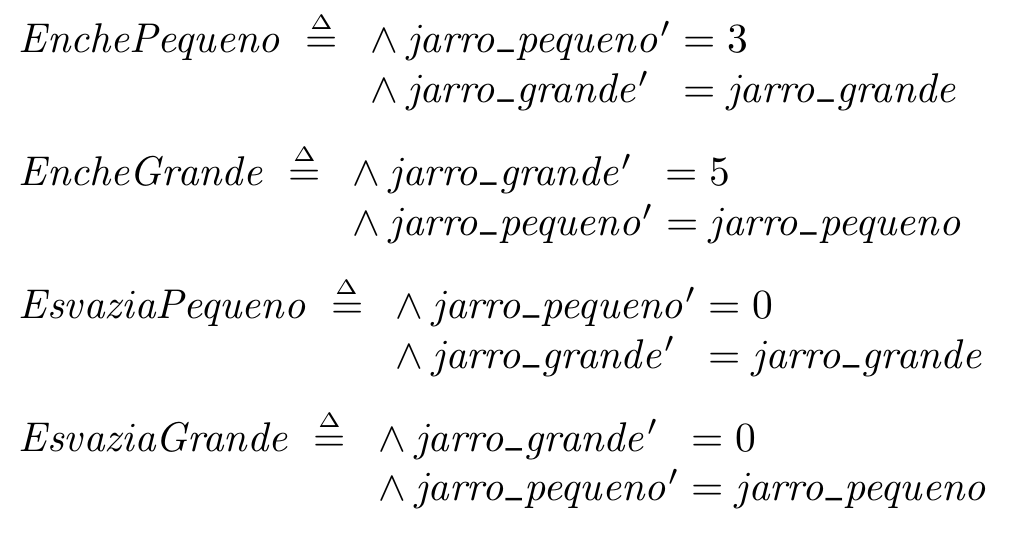
\includegraphics[width=0.6\textwidth]{JarrosP2.png}\\

         \TEqD\ (\texttt{DEF})\\

         \progfigmed{
         def enche\_pequeno\_condition(variables) do\\
         ~~True\\
         end\\\\
         def enche\_pequeno(variables) do\\
         ~~\%\{\\
         ~~~~jarro\_pequeno: 3,\\
         ~~~~jarro\_grande: variables[:jarro\_grande]\\
         ~~\}\\
         end\\
         ...
         }

       \end{array}$
     }}
   \caption{Tradução das definições simples dos Jarros de Água}
   \label{fig:jarros-ex-def1}
 \end{figure}

 \begin{figure}[h]
  \centering
  {\fbox{
      $\begin{array}{c}

         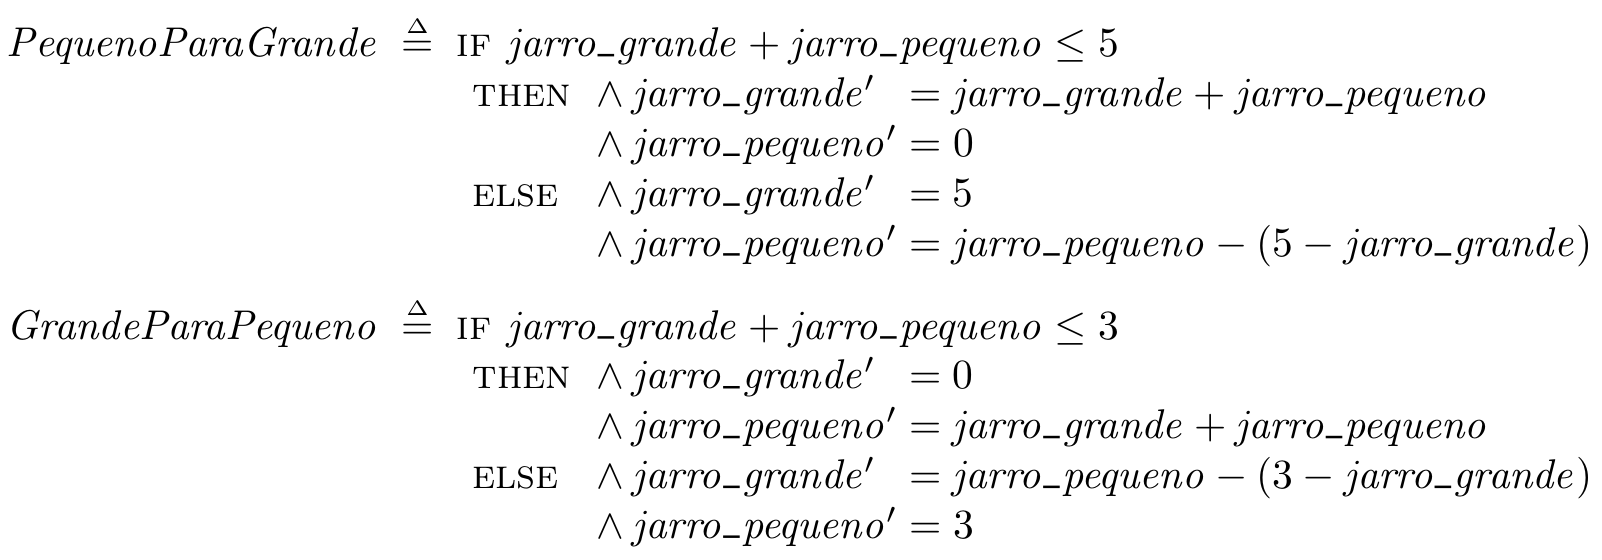
\includegraphics[width=0.9\textwidth]{JarrosP3.png}\\

         \TEqD\ (\texttt{DEF})\\

         \progfig{
         def pequeno\_para\_grande\_condition(variables) do\\
         ~~True\\
         end\\
         \\
         def pequeno\_para\_grande(variables) do\\
         ~~if variables[:jarro\_grande] + variables[:jarro\_pequeno] \textless{}= 5 do\\
         ~~~~\%\{\\
         ~~~~~~jarro\_grande:\ variables[:jarro\_grande] +\\
         ~~~~~~~~variables[:jarro\_pequeno],\\
         ~~~~~~jarro\_pequeno:\ 0\\
         ~~~~\}\\
         ~~else\\
         ~~~~\%\{\\
         ~~~~~~jarro\_grande:\ 5,\\
         ~~~~~~jarro\_pequeno:\ variables[:jarro\_pequeno] -\\
         ~~~~~~~~(5 - variables[:jarro\_grande])\\
         ~~~~\}\\
         ~~end\\
         end\\
         ...
         }
       \end{array}$
     }}
   \caption{Tradução das definições com condicionais dos Jarros de Água}
   \label{fig:jarros-ex-def2}
 \end{figure}

 \begin{figure}[h]
  \centering
  {\fbox{
      $\begin{array}{c}

         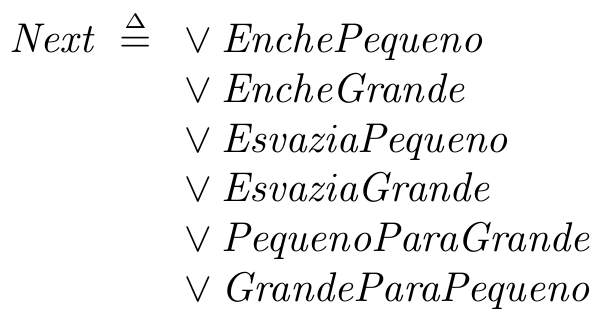
\includegraphics[width=0.4\textwidth]{JarrosP4.png}\\

         \TEqD\ (\texttt{NEXT})\\

         \progfig{
         def main(variables) do\\
         ~~IO.puts (inspect variables)\\
         \\
         ~~main(\\
         ~~~~decide\_action(\\
         ~~~~~~List.flatten([\\
         ~~~~~~~~\%\{\\
         ~~~~~~~~~~action: "EnchePequeno()",\\
         ~~~~~~~~~~condition: enche\_pequeno\_condition(variables),\\
         ~~~~~~~~~~state: enche\_pequeno(variables)\\
         ~~~~~~~~\},\\
         ~~~~~~~~\%\{\\
         ~~~~~~~~~~action: "EncheGrande()",\\
         ~~~~~~~~~~condition: enche\_grande\_condition(variables),\\
         ~~~~~~~~~~state: enche\_grande(variables)\\
         ~~~~~~~~\},\\
         ~~~~~~~~...\\
         ~~~~~~])\\
         ~~~~)\\
         ~~)\\
         end
         }
       \end{array}$
     }}
   \caption{Tradução da função de próximo estado para os Jarros de Água}
   \label{fig:jarros-ex-next}
 \end{figure}
